%!TEX program = xelatex+makeindex+bibtex
\documentclass[final]{scrreprt} %scrreprt of scrartcl
% Include all project wide packages here.
\usepackage{fullpage}
\usepackage{polyglossia}
\setmainlanguage{english}
\usepackage{csquotes}
\usepackage{graphicx}
\usepackage{epstopdf}
\usepackage{pdfpages}
\usepackage{caption}
\usepackage[list=true]{subcaption}
\usepackage{float}
\usepackage{standalone}
\usepackage{import}
\usepackage{tocloft}
\usepackage{wrapfig}
\usepackage{authblk}
\usepackage{array}
\usepackage{booktabs}
\usepackage[toc,page,title,titletoc]{appendix}
\usepackage{xunicode}
\usepackage{fontspec}
\usepackage{pgfplots}
\usepackage{SIunits}
\usepackage{units}
\pgfplotsset{compat=newest}
\pgfplotsset{plot coordinates/math parser=false}
\newlength\figureheight 
\newlength\figurewidth
\usepackage{amsmath}
\usepackage{mathtools}
\usepackage{unicode-math}
\usepackage[
    backend=bibtexu,
	texencoding=utf8,
bibencoding=utf8,
    style=ieee,
    sortlocale=en_US,
    language=auto
]{biblatex}
\usepackage{listings}
\newcommand{\includecode}[3][c]{\lstinputlisting[caption=#2, escapechar=, style=#1]{#3}}
\newcommand{\superscript}[1]{\ensuremath{^{\textrm{#1}}}}
\newcommand{\subscript}[1]{\ensuremath{_{\textrm{#1}}}}


\newcommand{\chapternumber}{\thechapter}
\renewcommand{\appendixname}{Bijlage}
\renewcommand{\appendixtocname}{Bijlagen}
\renewcommand{\appendixpagename}{Bijlagen}

\usepackage[hidelinks]{hyperref} %<--------ALTIJD ALS LAATSTE

\renewcommand{\familydefault}{\sfdefault}

\setmainfont[Ligatures=TeX]{Myriad Pro}
\setmathfont{Asana Math}
\setmonofont{Lucida Console}

\usepackage{titlesec, blindtext, color}
\definecolor{gray75}{gray}{0.75}
\newcommand{\hsp}{\hspace{20pt}}
\titleformat{\chapter}[hang]{\Huge\bfseries}{\chapternumber\hsp\textcolor{gray75}{|}\hsp}{0pt}{\Huge\bfseries}
\renewcommand{\familydefault}{\sfdefault}
\renewcommand{\arraystretch}{1.2}
\setlength\parindent{0pt}

%For code listings
\definecolor{black}{rgb}{0,0,0}
\definecolor{browntags}{rgb}{0.65,0.1,0.1}
\definecolor{bluestrings}{rgb}{0,0,1}
\definecolor{graycomments}{rgb}{0.4,0.4,0.4}
\definecolor{redkeywords}{rgb}{1,0,0}
\definecolor{bluekeywords}{rgb}{0.13,0.13,0.8}
\definecolor{greencomments}{rgb}{0,0.5,0}
\definecolor{redstrings}{rgb}{0.9,0,0}
\definecolor{purpleidentifiers}{rgb}{0.01,0,0.01}


\lstdefinestyle{csharp}{
language=[Sharp]C,
showspaces=false,
showtabs=false,
breaklines=true,
showstringspaces=false,
breakatwhitespace=true,
escapeinside={(*@}{@*)},
columns=fullflexible,
commentstyle=\color{greencomments},
keywordstyle=\color{bluekeywords}\bfseries,
stringstyle=\color{redstrings},
identifierstyle=\color{purpleidentifiers},
basicstyle=\ttfamily\small}

\lstdefinestyle{c}{
language=C,
showspaces=false,
showtabs=false,
breaklines=true,
showstringspaces=false,
breakatwhitespace=true,
escapeinside={(*@}{@*)},
columns=fullflexible,
commentstyle=\color{greencomments},
keywordstyle=\color{bluekeywords}\bfseries,
stringstyle=\color{redstrings},
identifierstyle=\color{purpleidentifiers},
}

\lstdefinestyle{matlab}{
language=Matlab,
showspaces=false,
showtabs=false,
breaklines=true,
showstringspaces=false,
breakatwhitespace=true,
escapeinside={(*@}{@*)},
columns=fullflexible,
commentstyle=\color{greencomments},
keywordstyle=\color{bluekeywords}\bfseries,
stringstyle=\color{redstrings},
identifierstyle=\color{purpleidentifiers}
}

\lstdefinestyle{vhdl}{
language=VHDL,
showspaces=false,
showtabs=false,
breaklines=true,
showstringspaces=false,
breakatwhitespace=true,
escapeinside={(*@}{@*)},
columns=fullflexible,
commentstyle=\color{greencomments},
keywordstyle=\color{bluekeywords}\bfseries,
stringstyle=\color{redstrings},
identifierstyle=\color{purpleidentifiers}
}

\lstdefinestyle{xaml}{
language=XML,
showspaces=false,
showtabs=false,
breaklines=true,
showstringspaces=false,
breakatwhitespace=true,
escapeinside={(*@}{@*)},
columns=fullflexible,
commentstyle=\color{greencomments},
keywordstyle=\color{redkeywords},
stringstyle=\color{bluestrings},
tagstyle=\color{browntags},
morestring=[b]",
  morecomment=[s]{<?}{?>},
  morekeywords={xmlns,version,typex:AsyncRecords,x:Arguments,x:Boolean,x:Byte,x:Char,x:Class,x:ClassAttributes,x:ClassModifier,x:Code,x:ConnectionId,x:Decimal,x:Double,x:FactoryMethod,x:FieldModifier,x:Int16,x:Int32,x:Int64,x:Key,x:Members,x:Name,x:Object,x:Property,x:Shared,x:Single,x:String,x:Subclass,x:SynchronousMode,x:TimeSpan,x:TypeArguments,x:Uid,x:Uri,x:XData,Grid.Column,Grid.ColumnSpan,Click,ClipToBounds,Content,DropDownOpened,FontSize,Foreground,Header,Height,HorizontalAlignment,HorizontalContentAlignment,IsCancel,IsDefault,IsEnabled,IsSelected,Margin,MinHeight,MinWidth,Padding,SnapsToDevicePixels,Target,TextWrapping,Title,VerticalAlignment,VerticalContentAlignment,Width,WindowStartupLocation,Binding,Mode,OneWay,xmlns:x}
}

%defaults
\lstset{
basicstyle=\ttfamily\small,
extendedchars=false,
numbers=left,
numberstyle=\ttfamily\tiny,
stepnumber=1,
tabsize=4,
numbersep=5pt
}
\addbibresource{../../library/bibliography.bib}

\begin{document}

\chapter{Task 3}

\section{Experimental procedure}
\label{sec:experimentalprocedure}
The range resolution of the radar demonstrator is determined in this experiment.
This can be done by finding the minimum distance for which a radar's indicator still identifies two different targets. 
We got two reference targets that we had to place in the radar's line of sight.
If one target is fixed we change the position of the second target until a minimum distance is reached for which the radar's indicator still identifies two targets.
Starting with the two targets next to each other we slowly moved the second one back a little until we saw two different waves on the monitor.
When the second wave appears on the monitor the distance between the two targets is measured and the minimum distance is found.
This minimum distance is called $\Delta R$ and can also be found using equation \ref{eq:1}. 
In this equation $c_{0}$ is the speed of light and $B$ is the bandwidth of the system.
In our experiment the bandwidth was between 0 and 26 $\giga Hz$. 
\begin{equation} 
\label{eq:1}
\Delta R= \frac{c_{0}}{2B} 
\end{equation}
The setup of our experiment can be seen in figure \ref{fig:range}
\begin{figure}[h]
	\begin{center}
		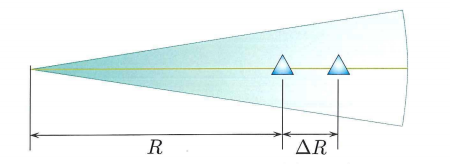
\includegraphics[width=\linewidth/2]{resources/meet3.png}
	\end{center}
	\caption{Range resolution experiment}
	\label{fig:range}
\end{figure}


\section{Results}
We did the experiment at several distances from the radar: 2.00 \unit{m}, 2.50 \unit{m}, 3.50 \unit{m}, 5.00 \unit{m} and 5.50 \unit{m}. 
With the results found for $\Delta R$ we can calculate the Bandwidth $B$ from equation \ref{eq:1}.
The results from the experiment are shown in Table \ref{tab:2}
\begin{table}[h]
\begin{center}
\begin{tabular}{ | l | l | l | }
    \hline
    Distance between radar and object R (m) & Minimum distance $\Delta R$ (cm) & Bandwidth ($\giga Hz$)  \\\hline
    2.00 & 0.50 & 30.0 \\\hline
    2.50 & 0.50 & 30.0 \\\hline
    3.50 & 0.75 & 20.0  \\\hline
    5.00 & 1.00 & 15.0  \\\hline
    5.50 & 1.00 & 15.0  \\\hline
\end{tabular}
\caption{Measure data range resolution experiment.}
\label{tab:2}
\end{center}
\end{table}
\\


Analyzing the results we've got from the experiment we see that the minimum distance becomes just a little bigger when the distance between the radar and the targets becomes larger.
We also see that the bandwidth at 2.00 \unit{m} and 2.50 \unit{m} is 30.0 $\giga Hz$ and exceeds the specified region in \ref{sec:experimentalprocedure}.
This could be because:
\begin{itemize}
\item we did not measure $\Delta R$ correctly. 
Due to the small distance between the two targets and due to measuring by hand ,the measured value can be off. 
With a slightly bigger $\Delta R$, 0.60 \unit{\centi m} for example, the bandwidth becomes  25.0 $\giga Hz$,  which is in fact within the specified region.
\item it was recommendable to locate the target at a distance of at least 5.00 \unit{m} to minimize the wave propagation effect and circumvent some equipment non-idealities.
 So the farther is better.
\end{itemize}


\end{document}